\section{Визуализация и тестирование}

\begin{tabular}{| l | l |}
    \hline
    \textbf{Тест} & \textbf{Описание} \\
    \hline
    int counter; & Примитивный тест с одним простым описанием. \\
    \hline
    int counter & Тест, в котором забыли про точку с запятой. \\
    \hline
    , counter; & Тест, в котором вместо имени типа запятая. \\
    \hline
    int counter; char c; & Тест с двумя описаниями. \\
    \hline
    int counter; char @ c; & Во втором описании неизвестный символ. \\
    \hline
    size\_t counter;  & Подчёркивание в имени типа. \\
    \hline
    int 9thousands;  & Имя не может начинаться с цифры. \\
    \hline
    line2 counter2;  & Но цифра может быть в имени. \\
    \hline
    size\_t counter, index\_of\_string;  & Несколько переменных. \\
    \hline
    char * buf, ** point\_to\_str, cur\_char;  & Указатели. \\
    \hline
    void buf *;  & Не в том месте звёздочка. \\
    \hline
    point\_3t * pointer, p, ** * * o\_O; void * buf, ** a;  & Большой тест. \\
    \hline
    point\_3t * pointer, p, ** * * o\_O; void * buf ** a;  & Забыли запятую. \\
    \hline
\end{tabular}

\subsection{Результаты тестов}

\subsubsection{Тест 1}
int counter;

Passed.
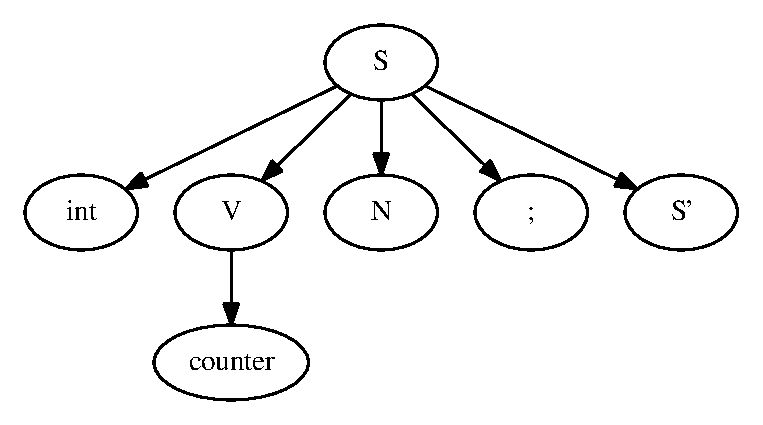
\includegraphics[width=\textwidth]{graph1.eps}

\subsubsection{Тест 2}
int counter

Failed.
Wrong input format at position 12, comma or semicolon was expected, but end of file was found

\subsubsection{Тест 3}
, counter;

Failed.
Wrong input format at position 0, name was expected, but , was found

\subsubsection{Тест 4}
int counter; char c;

Passed.
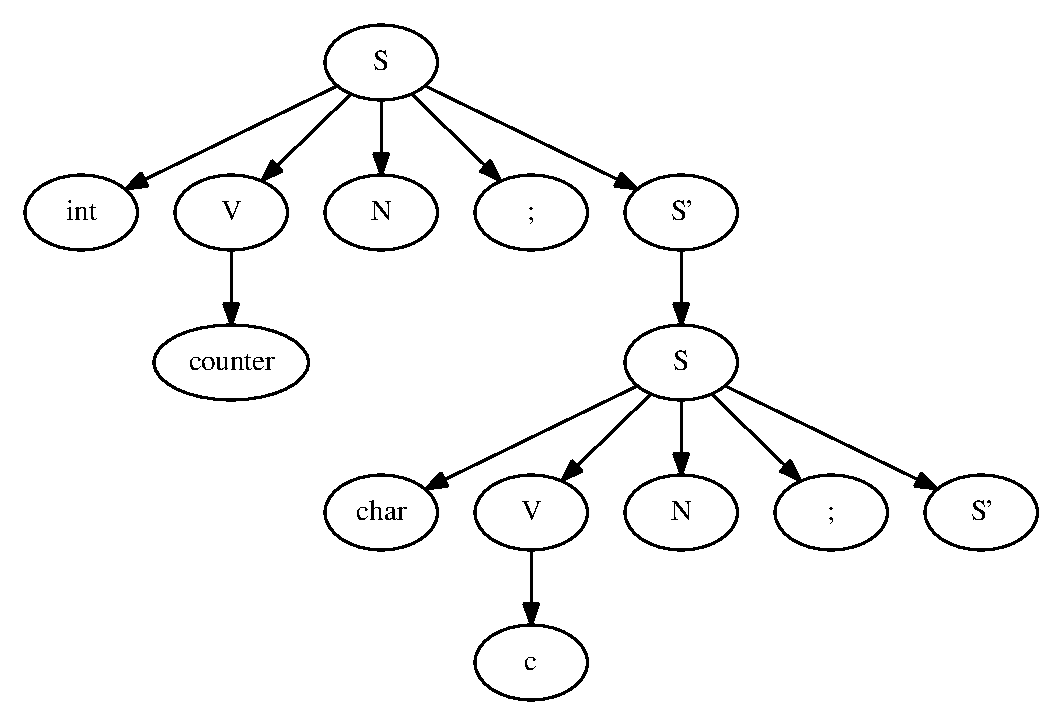
\includegraphics[width=\textwidth]{graph4.eps}

\subsubsection{Тест 5}
int counter; char @ c;

Failed.
Parsing error. Bad symbol at position 18

\subsubsection{Тест 6}
size\_t counter;

Passed.
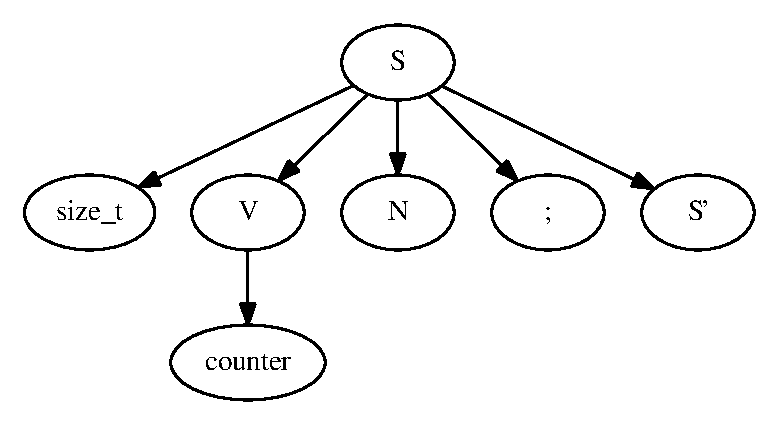
\includegraphics[width=\textwidth]{graph6.eps}

\subsubsection{Тест 7}
int 9thousands;

Failed.
Parsing error. Bad symbol at position 4

\subsubsection{Тест 8}
line2 counter2;

Passed.
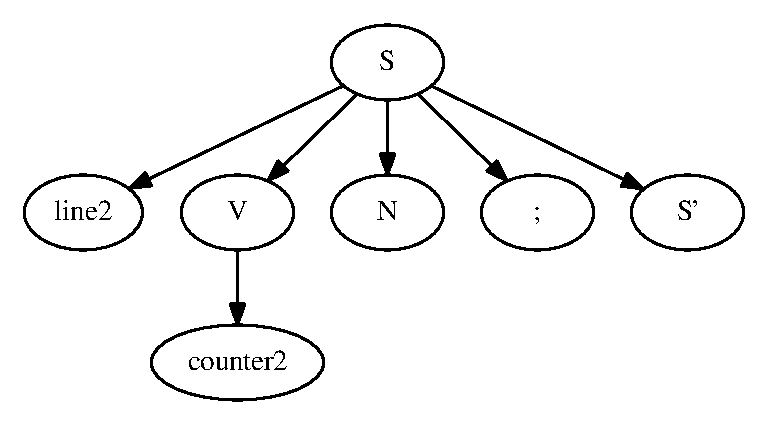
\includegraphics[width=\textwidth]{graph8.eps}

\subsubsection{Тест 9}
size\_t counter, index\_of\_string;

Passed.
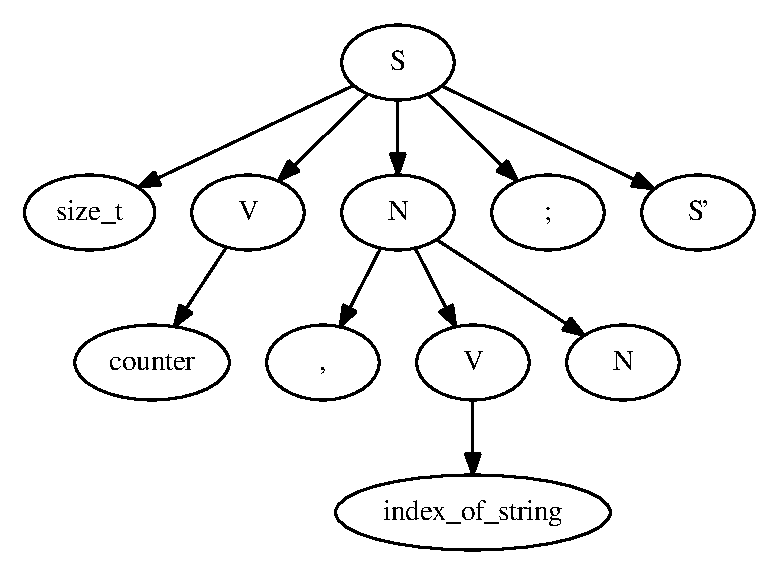
\includegraphics[width=\textwidth]{graph9.eps}

\subsubsection{Тест 10}
char * buf, ** point\_to\_str, cur\_char;

Passed.
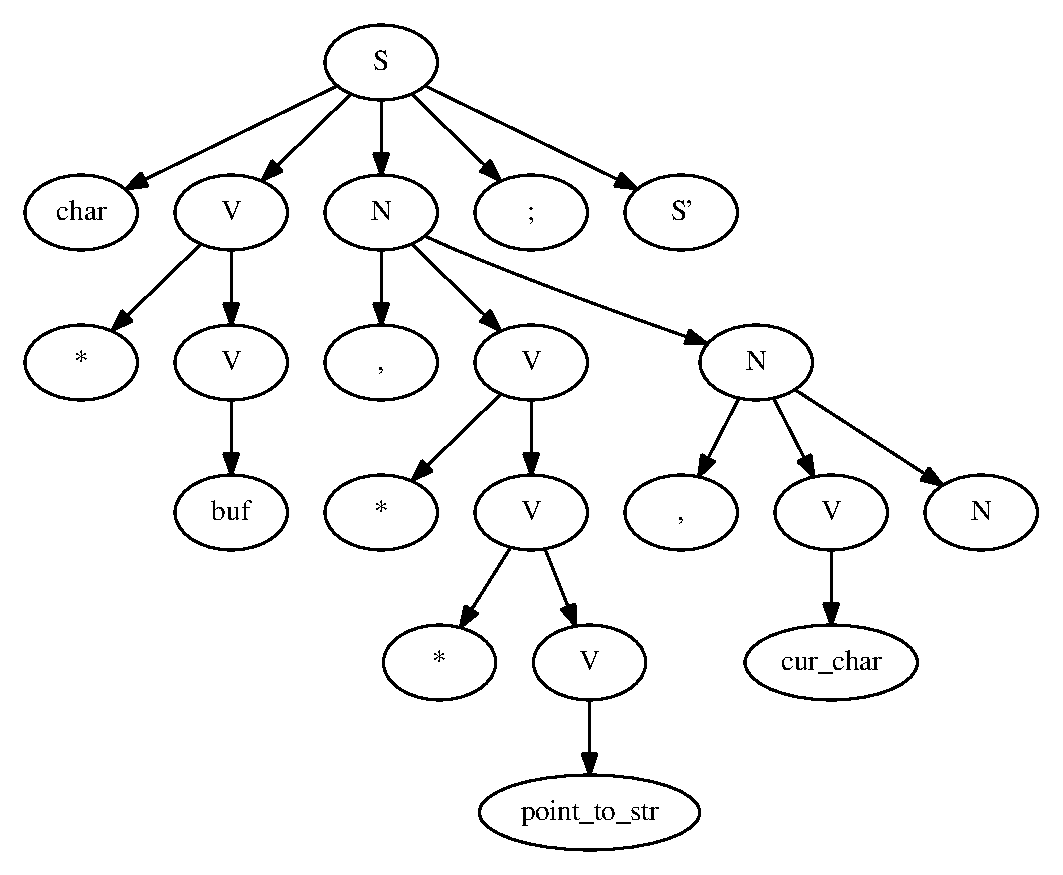
\includegraphics[width=\textwidth]{graph10.eps}

\subsubsection{Тест 11}
void buf *;

Failed.
Wrong input format at position 9, comma or semicolon was expected, but * was found

\subsubsection{Тест 12}
point\_3t * pointer, p, ** * * o\_O; void * buf, ** a;

Passed.
\includegraphics[width=\textwidth]{graph12.eps}

\subsubsection{Тест 13}
point\_3t * pointer, p, ** * * o\_O; void * buf ** a;

Failed.
Wrong input format at position 46, comma or semicolon was expected, but * was found

